% DYNGEN CONTENT

\begin{quote}
	\textbf{Abstract:} 
\end{quote}

\section{Introduction}
Continuous technological advancements to single-cells omics are having profound 
effects on how researchers can validate biological hypotheses. 
Early experimental technologies typically only allowed profiling a single modality (e.g. DNA sequence, 
RNA or protein expression). However, recent developments permit profiling multiple modalities simultaneously,
and every modality added allows for new types of analyses that can be performed.

This presents method developers with a problem. The majority of the 250+ peer-reviewed computational tools for analysing single cell omics data were published without a quantitative assessment of the accuracy of the tool. This is partially due to low availability of suitable benchmarking datasets; even if there are sufficient suitable input datasets available, these are often not accompanied by the necessary metadata to serve as ground-truth for a benchmark.

Here, synthetic data plays a crucial role in asserting minimum performance requirements for novel tools in anticipation of adequate real data. Generators of scRNA-seq data (e.g. splatter \cite{zappia_splattersimulationsinglecell_2017}, powsimR \cite{vieth_powsimrpoweranalysis_2017}, PROSSTT \cite{papadopoulos_prossttprobabilisticsimulation_2018} and SymSim \cite{zhang_simulatingmultiplefaceted_2019}) have already been widely used to explore the strengths and weakness of computational tools, both by method developers\cite{street_slingshotcelllineage_2018,parra_reconstructingcomplexlineage_2018,lummertzdarocha_reconstructioncomplexsinglecell_2018,lin_scclassifyhierarchicalclassification_2019} and independent benchmarkers\cite{duo_systematicperformanceevaluation_2018,saelens_comparisonsinglecelltrajectory_2019,soneson_biasrobustnessscalability_2018}.
However, a limitation of scRNA-seq profiles generators is that they would require significant methodological alterations to add additional modalities.

An ideal experiment would be able to observe all aspects of a cell, including a full history of its 
molecular states, spatial positions and environmental interactions \cite{stuart_integrativesinglecellanalysis_2019}.
While this falls outside the reach of current experimental technologies, generating synthetic data in anticipation of new experimental technologies would allow already developing the next wave of computational tools.

We introduce \texttt{dyngen}, a multi-modality simulator of single cells and their dynamics (Figure \ref{fig:showcase}A). A cell is simulated using Gillespie's Stochastic Simulation Algorithm (SSA) \cite{gillespie_exactstochasticsimulation_1977} where a cell consists of a set of molecules. Throughout a simulation, reactions (e.g. transcription, splicing) modify the abundance of these molecules, and the likelihood of a reaction occurring is again dependent on molecule abundance.

By simulating a cell over time in terms of its molecular state and the reactions that are allowed to occur, the simulator is more extendible to new modalities or experimental procedures (Figure~\ref{fig:showcase}B). We demonstrate \texttt{dyngen}'s flexibility by simulating three different types of biological experiments, and using these simulations to develop benchmarking methodologies for recently developed computational tools.

\begin{figure}[htb!]
	\centering
	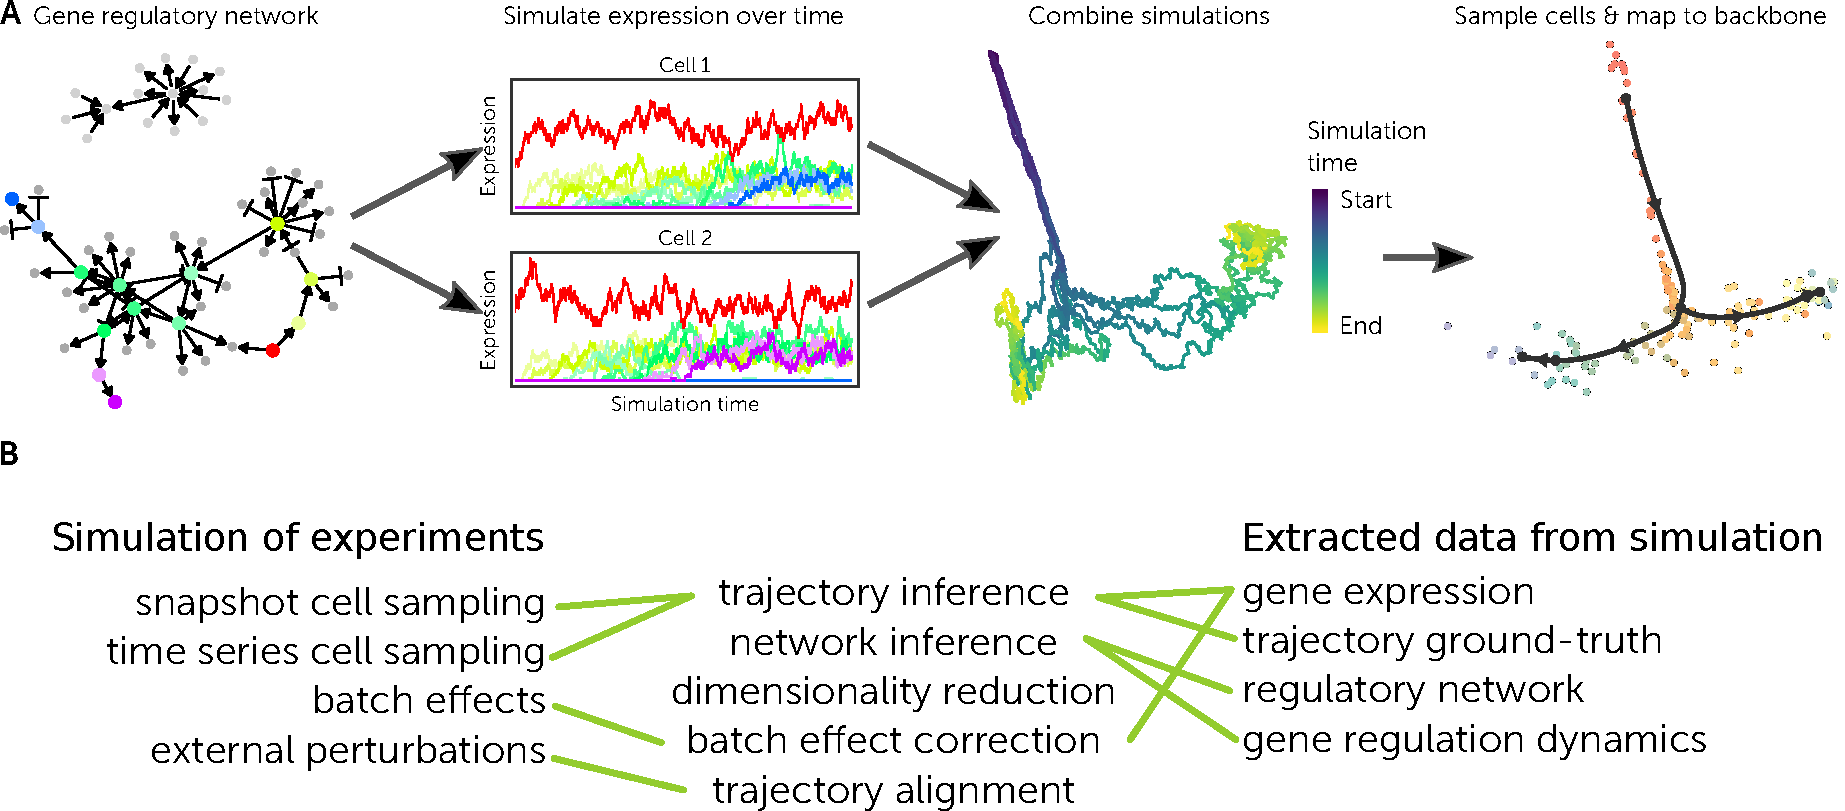
\includegraphics[width=\linewidth]{fig/showcase_4} 
	\caption{
		\textbf{Showcase of \texttt{dyngen} functionality.} 
		\textbf{A:} 
		\textbf{B:} Evaluating different types of computational tools requires simulating different types of experiments and extracting different layers of information from the simulation.
	}
	\label{fig:showcase}
\end{figure}

\section{Results}

A cell consists of a set of molecules, the abundance of which are affected by a set of reactions: transcription, splicing, translation, and degradation (Figure \ref{fig:simplecyclic}A). 
A gene regulatory network (GRN) define the reactions that are allowed to occur (Figure \ref{fig:simplecyclic}B), and is constructed such that a cell will develop over time (Figure \ref{fig:simplecyclic}C--D).
The likelihood of a reaction occurring is a function of the abundance of key molecules involved in each reaction (Figure \ref{fig:simplecyclic}E).

\begin{figure}[htb!]
	\centering
	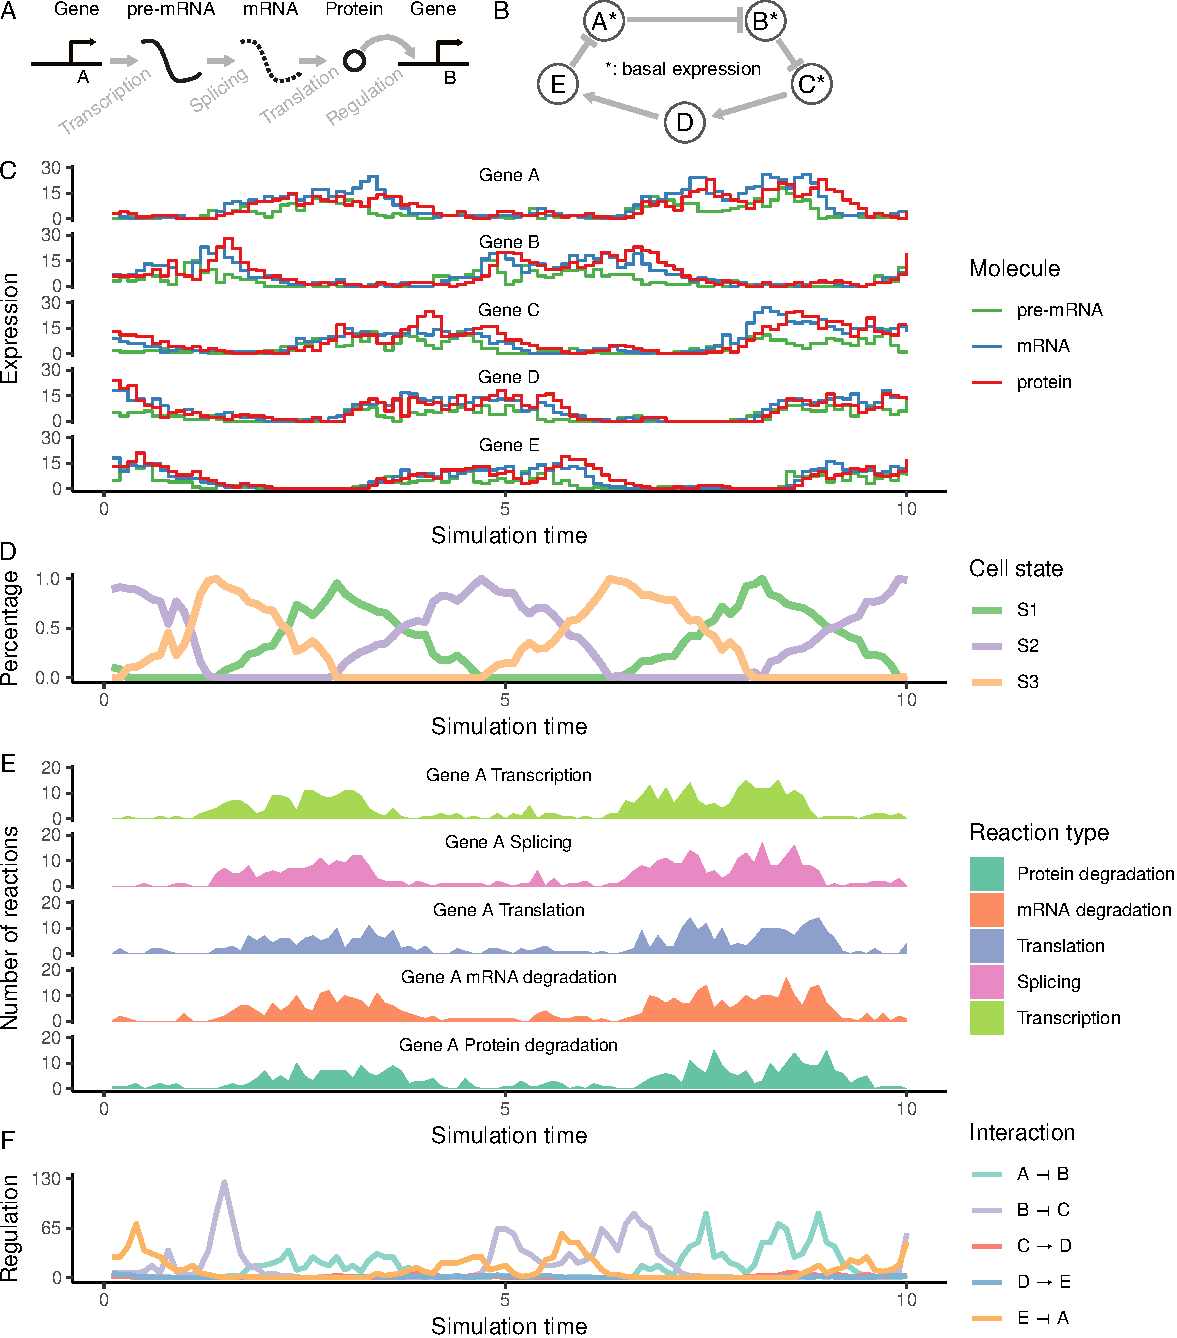
\includegraphics[width=\linewidth]{fig/simplecyclic_edited} 
	\caption{
		\textbf{Key features of \texttt{dyngen} are illustrated using a cyclic toy example.}
		While this example comprises only of a single cell and 5 genes, \texttt{dyngen} is able to simulate thousands of cells with GRNs containing thousands of genes.
	}
	\label{fig:simplecyclic}
\end{figure}

\texttt{dyngen} returns many modalities throughout the whole simulation: molecular abundance, cellular state, number of reaction firings, reaction likelihoods, and regulation activations (Figure \ref{fig:simplecyclic}C--F). These modalities can serve both as input data and ground truth for benchmarking many types of computational approaches. For example, a network inference method could use mRNA abundance and cellular states as inputs, and its output could be benchmarked against the gold standard GRN.

Depending on how the GRN is designed, different cellular developmental processes can be simulated.
\texttt{dyngen} includes generators of GRNs which result in many different developmental topologies (Figure~\ref{fig:example_runs}), including branching, converging, cyclic and even disconnected.

\begin{figure}[ht]
	\centering
	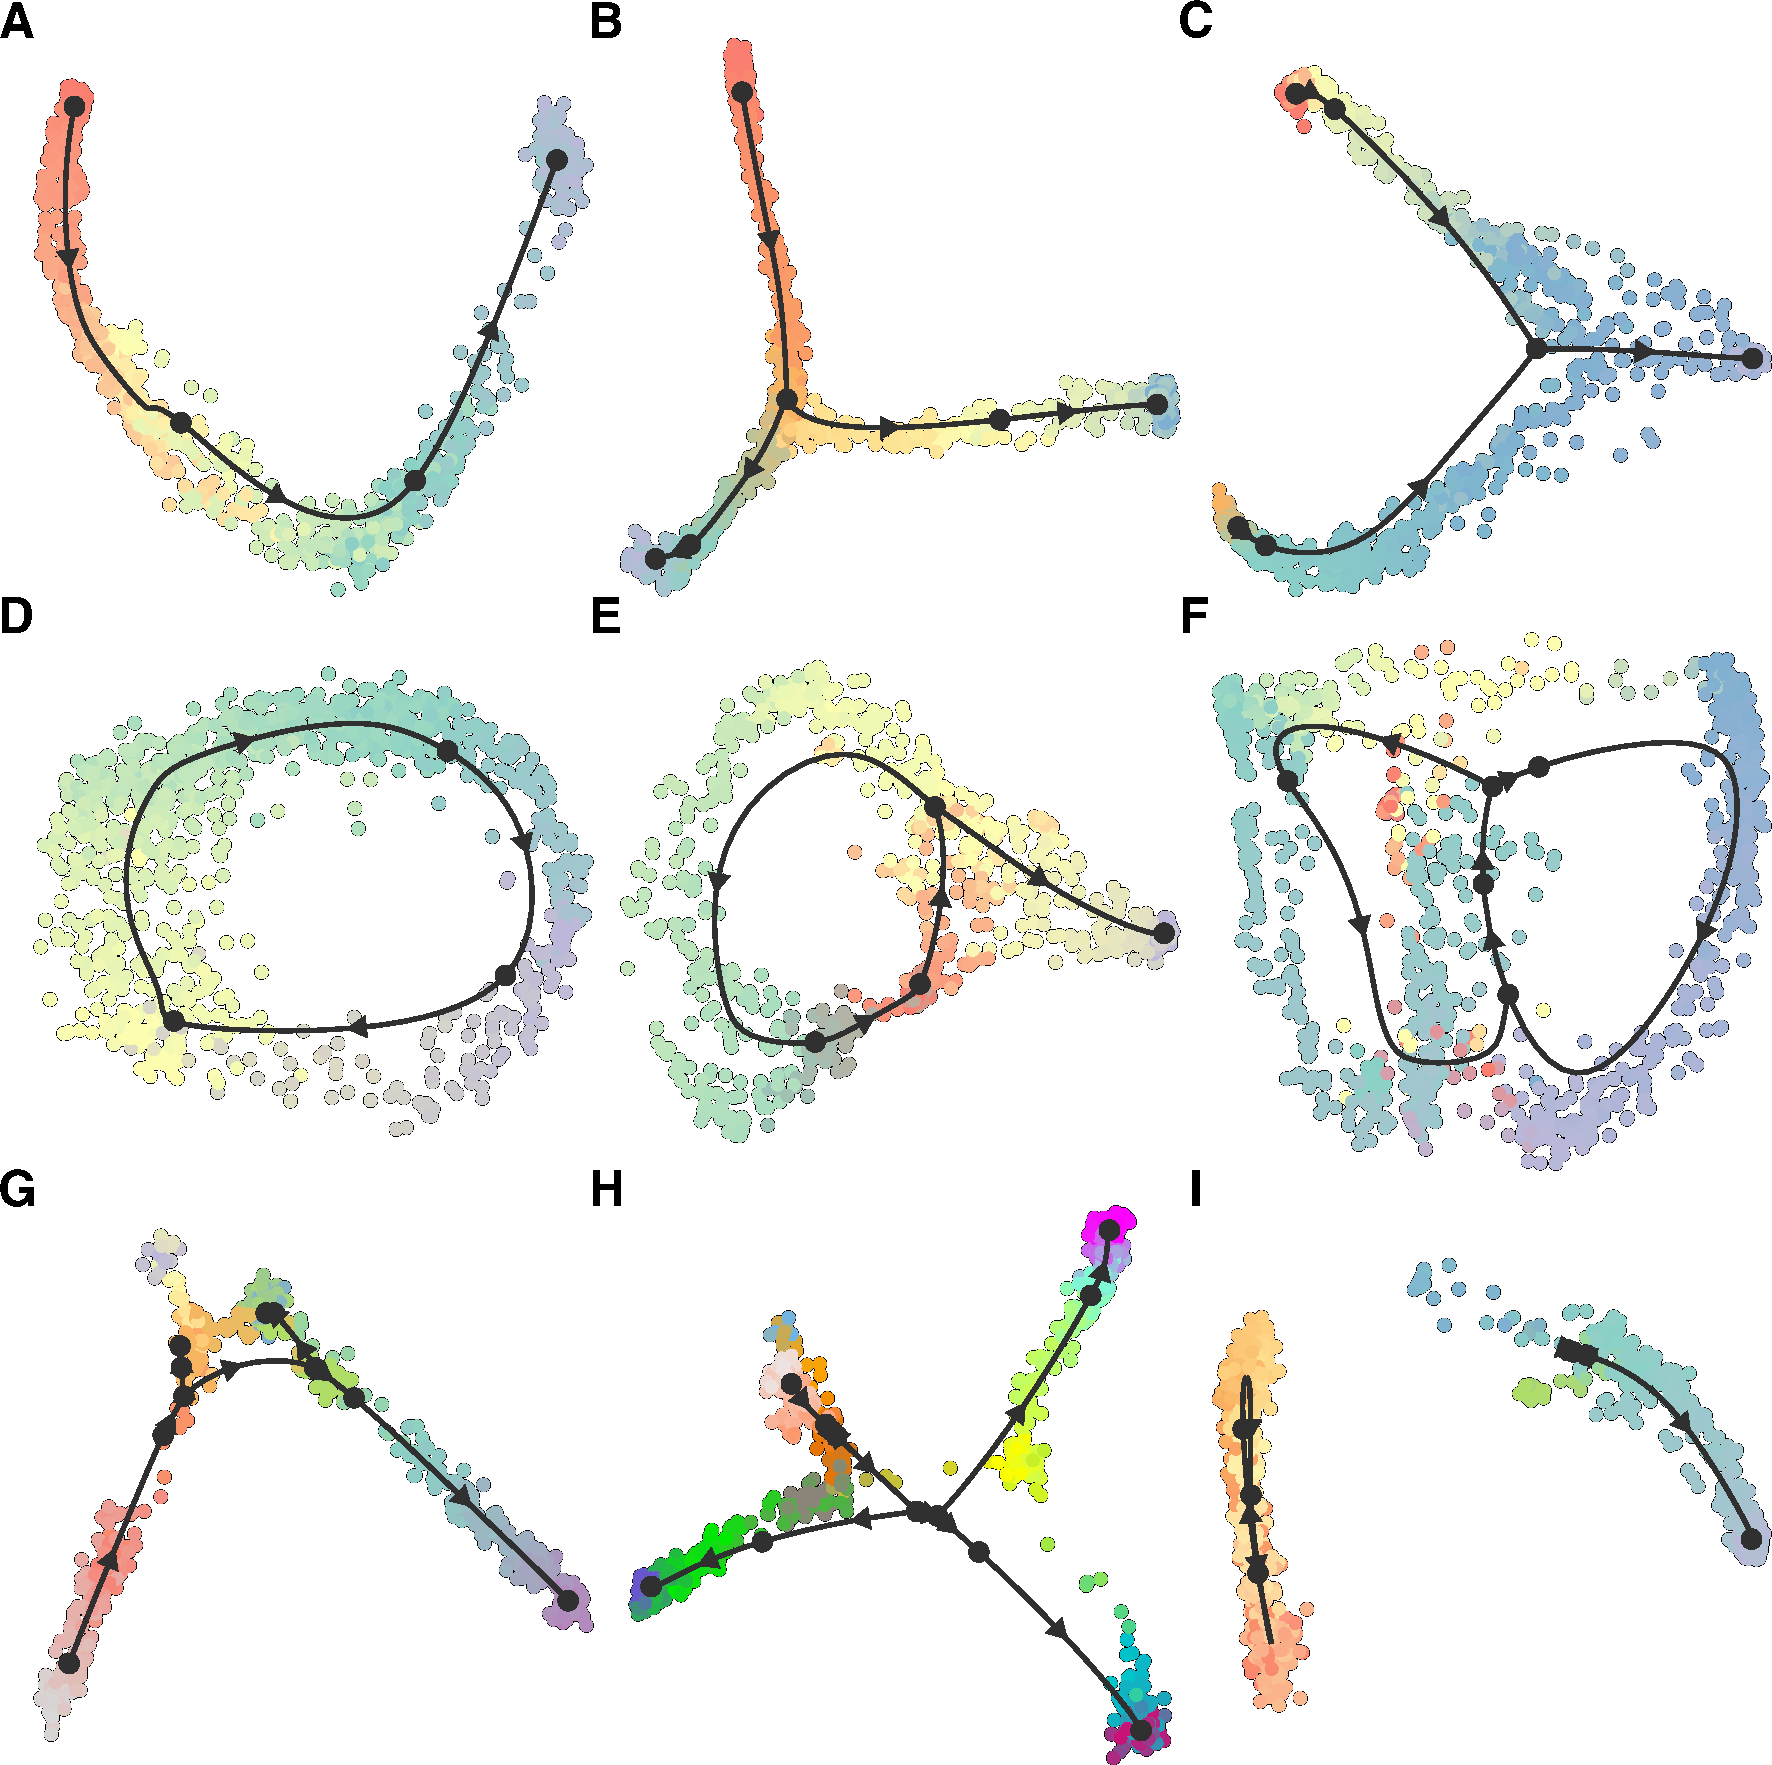
\includegraphics[width=\LARgefigure]{fig/example_runs_2} 
	\caption{
		\textbf{Multiple executions of \texttt{dyngen} with different predefined backbones.} From each simulation of about 200 genes, 1000 cells were sampled. 
		\textbf{A:}~Linear. \textbf{B:}~Bifurcating. \textbf{C:}~Converging.
		\textbf{D:}~Cyclic. \textbf{E:}~Bifurcating loop. \textbf{F:}~Bifurcating converging.
		\textbf{G:}~Consecutive branching. \textbf{H:}~Binary tree. \textbf{I:}~Disconnected.
	}
	\label{fig:example_runs}
\end{figure}

Custom-defined GRNs offer more fine-grained control over the simulation.
Aside from simulating topologies currently not supported by \texttt{dyngen}, this has several other important use-cases. Simulations of the same GRN with small perturbations allow to emulate batch effects or perturbation experiments (Figure~\ref{fig:usecases}). 
Simulating perturbed GRNs allow evaluating trajectory alignment methods -- which attempt to map two or more trajectories onto each other -- or differential network inference methods -- which infer differential regulatory interactions between two or more groups of profiles.


\begin{figure}[ht]
	\centering
	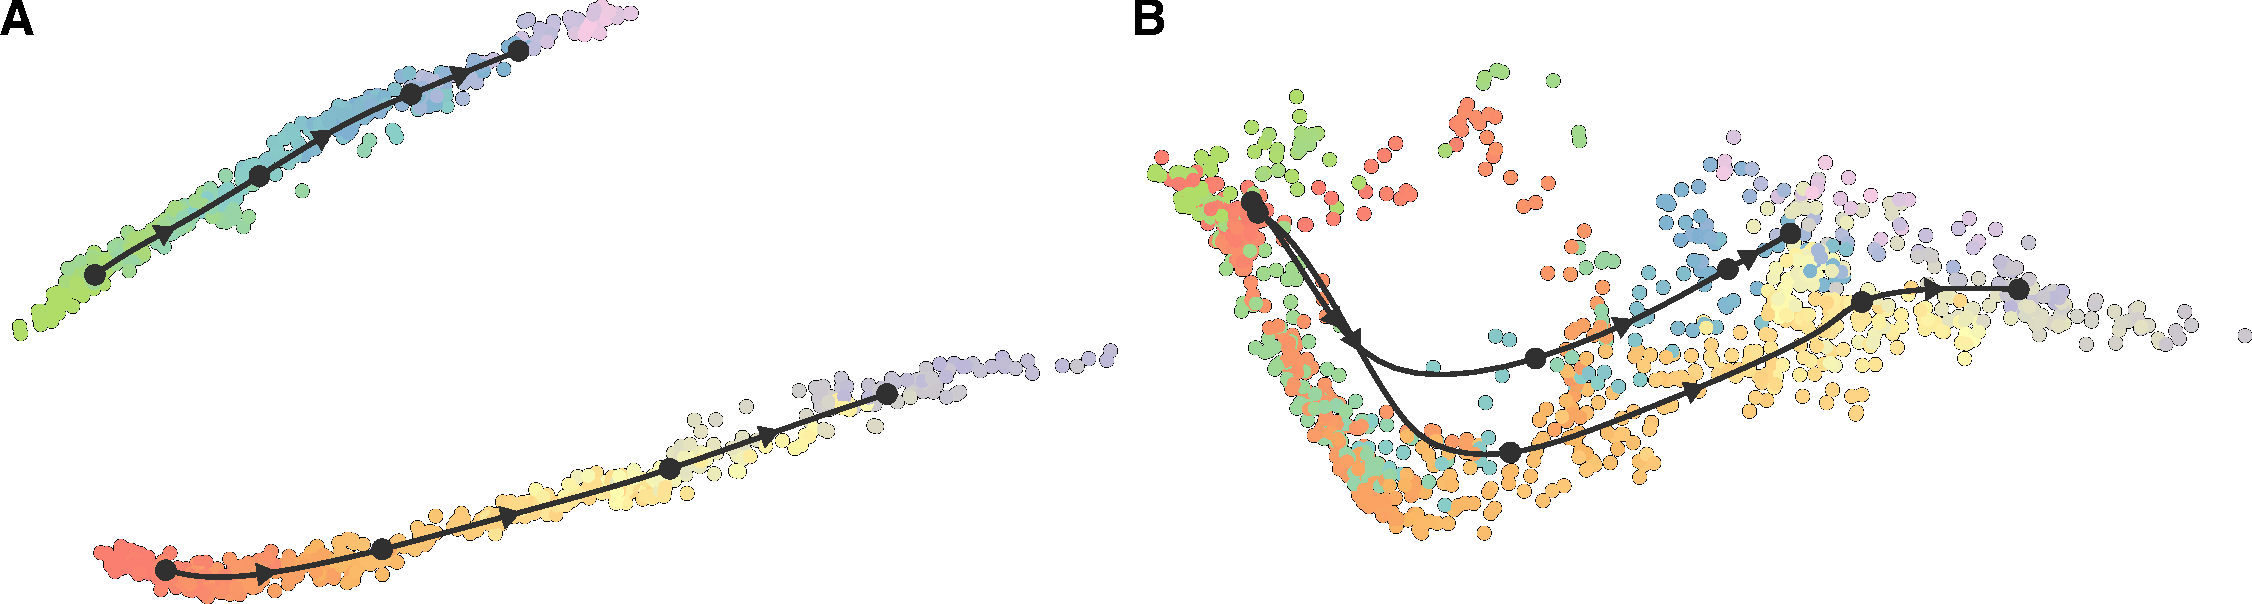
\includegraphics[width=\LARgefigure]{fig/usecases} 
	\caption{
		\textbf{Examples of simulations with perturbed GRNs.}  
		\textbf{A:} The cells in the top half were simulated with the same GRN as the cells on the bottom half, except that all parameters (e.g. strength of the interaction) were randomised.
		\textbf{B:} Only 10 interactions in the GRN were randomised. In this example, the effect of the GRN perturbation is more subtle.
	}
	\label{fig:usecases}
\end{figure}

\texttt{dyngen} can be used to simulate different experimental conditions. By default, \texttt{dyngen} supports snapshot experiments (uniformly sampling from an asynchronous dynamic process) and time-series experiments (sampling cells from different intervals in the simulation). 
However, it is possible to imagine and implement other sampling strategies, such as sampling a cell at a certain time point and once more at a later time point. This would allow evaluating the performance of RNA velocity approaches -- which predict the future state of a cell by looking at differences in pre-mRNA and mRNA abundance levels.

%\subsection{Example use cases}
%\subsubsection{Trajectory alignment}
%\subsubsection{Differential network inference}
%\subsubsection{RNA velocity}
%\subsubsection{Perturbation experiment}

\section{Discussion}
As is, \texttt{dyngen}'s single cell simulations can be used to evaluate common single-cell omics computational methods such as clustering, batch correction, trajectory inference and network inference.
However, the combined effect of these advantages results in a framework that is flexible enough to adapt to a broad range of applications. This may include methods that integrate clustering, network inference and trajectory inference. In this respect, \texttt{dyngen} may promote the development of new tools in the single-cell field similarly as other simulators have done in the past \cite{schaffter_genenetweaversilicobenchmark_2011,ewing_combiningtumorgenome_2015}.

\texttt{dyngen} ultimately allows anticipating technological developments in single-cell multi-omics. In this way, it is possible to design and evaluate the performance and robustness of new types of computational analyses before experimental data becomes available.
In addition, it could also be used to compare which experimental protocol is the most cost-effective in producing the qualitative and robust results in downstream analysis.

Currently, \texttt{dyngen} focuses on simulating cells as standalone entities that are well mixed.
Splitting up the simulation space into separate subvolumes could pave the way to better study key cellular processes such as cell division, intercellular communication and migration\cite{smith_spatialstochasticintracellular_2019}.


\section{Methods}
The workflow to generate \textit{in silico} single cell data consists of six main steps (Figure \ref{fig:explain_methods}). 

\begin{figure}[htb!]
	\centering
	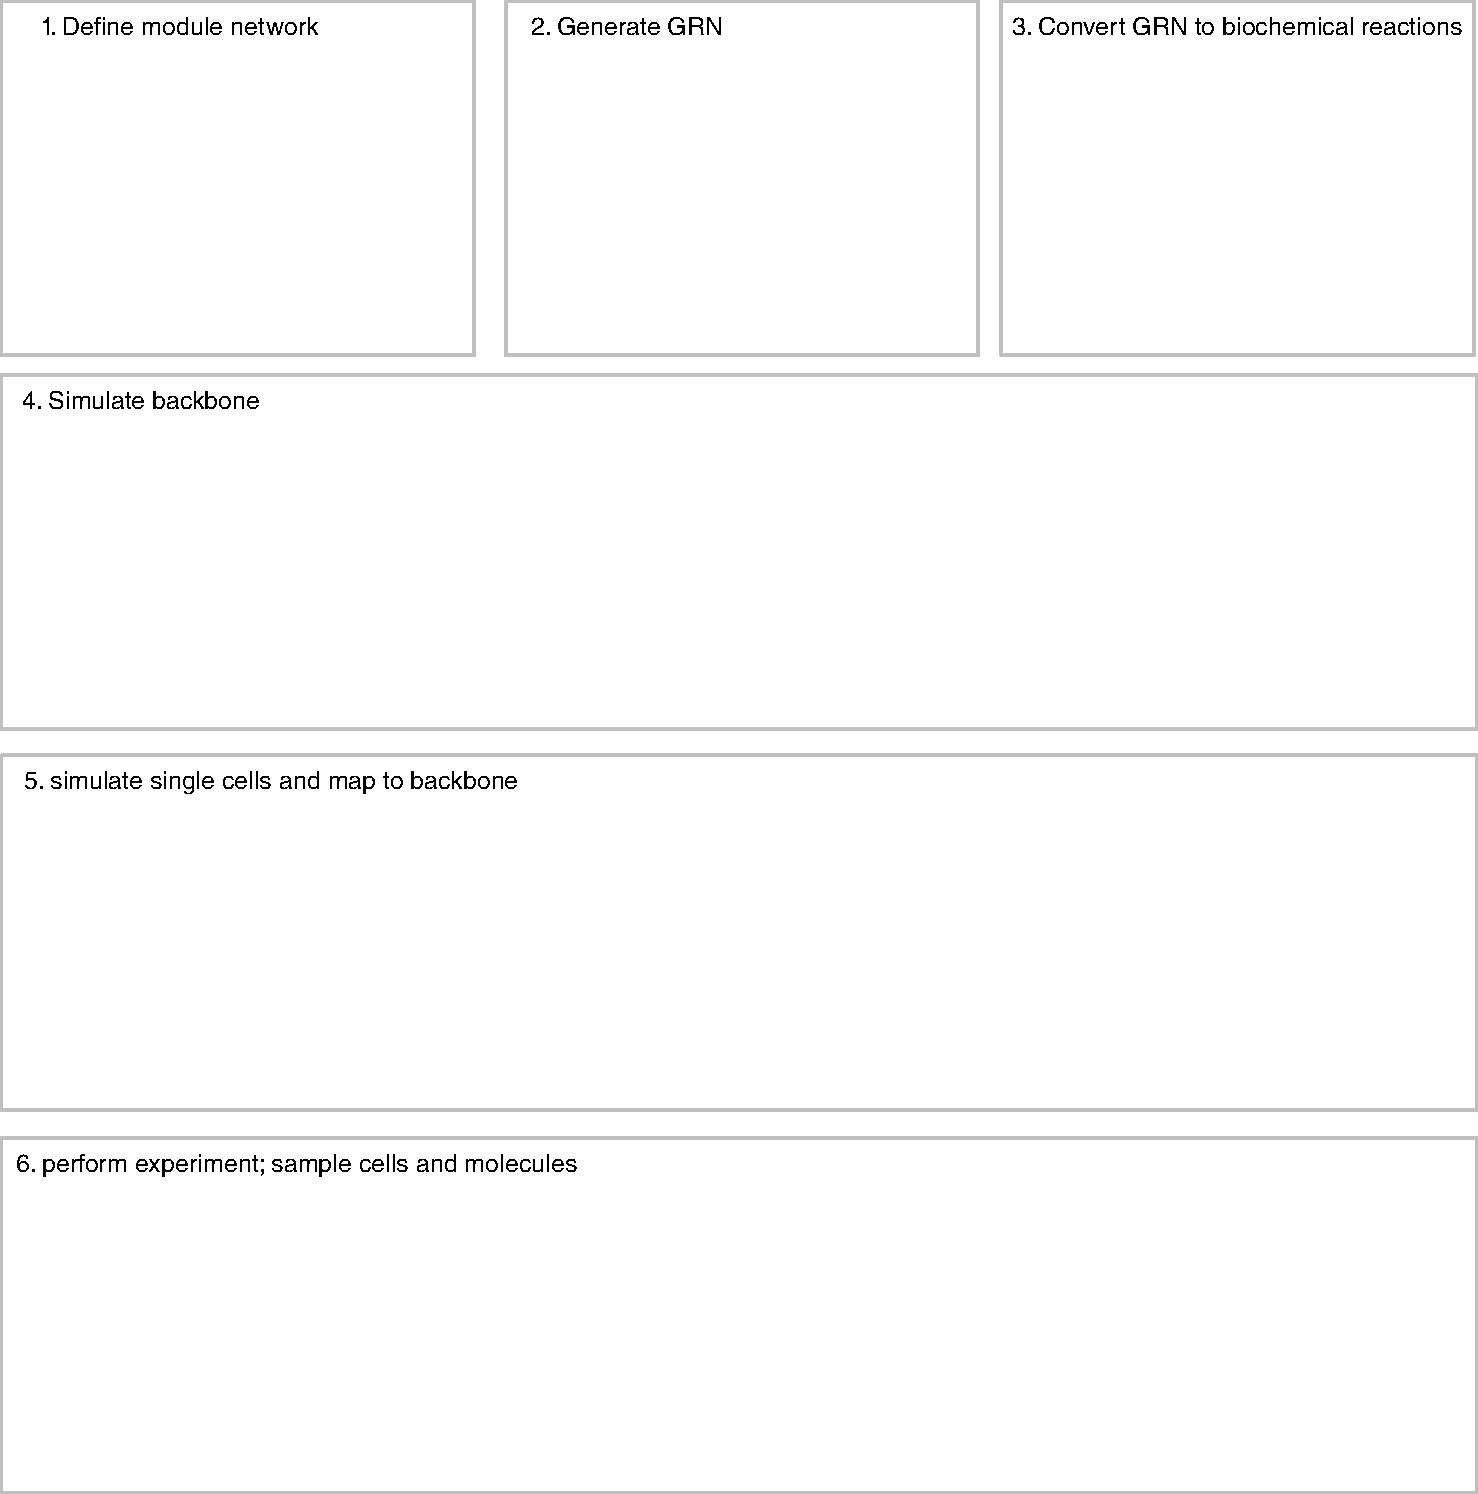
\includegraphics[width=\hugefigure]{fig/explain_methods} 
	\caption{\textbf{The workflow of \texttt{dyngen} is comprised of six main steps.} \textbf{A:} The user needs to specify the desired module network or use a predefined module network. \textbf{B:} Each gene in a module is is regulated by one or more transcription factors from the upstream module. Additional target genes are generated. \textbf{C:} Each gene regulatory interaction in the GRN is converted to a set of biochemical reactions. \textbf{D:} Along with the module network, the user also needs to specify the backbone structure of expected cell states. The average expression of each edge in the backbone is simulated by activating a restricted set of genes for each edge. \textbf{E:} Multiple Gillespie SSA simulations are run using the reactions defined in step C.  The counts of each of the mocules at each time step are extracted. Each time step is mapped to a point in the backbone. \textbf{F:} Multiple cells are sampled from each simulation. Molecules are sampled from each cell.}
	\label{fig:explain_methods}
\end{figure}

\subsection{Defining the backbone: modules and states} \label{sec:backbone}

One of the main processes involved in cellular dynamic processes is gene regulation, where regulatory cascades and feedback loops lead to progressive changes in expression and decision making. The exact way a cell chooses a certain path during its differentiation is still an active research field, although certain models have already emerged and been tested \textit{in vivo}. One driver of bifurcation seems to be mutual antagonism, where two genes \cite{xu_regulationbifurcatingcell_2015} strongly repress each other, forcing one of the two to become inactive \cite{graf_forcingcellschange_2009}. Such mutual antagonism can be modelled and simulated \cite{wang_quantifyingwaddingtonlandscape_2011, ferrell_bistabilitybifurcationswaddington_2012}. Although the two-gene model is simple and elegant, the reality is frequently more complex, with multiple genes (grouped into modules) repressing each other \cite{yosef_dynamicregulatorynetwork_2013}.

In \texttt{dyngen}, the user defines the behaviour of the simulation by defining how sets of genes, called modules, are regulating eachother.
A module may have basal expression, which means that pre-mRNA of the genes in this module will be transcribed without the presence of transcription factor molecules. A module marked as "active during the burn phase" means that this module will be allowed to generate expression of its genes during an initial warm-up phase (See section \ref{sec:dyngen_ssa}). At the end of the \texttt{dyngen} process, cells will not be sampled from the burn phase simulations. Interactions between modules have a strength (which is a positive integer) and an effect (+1 for upregulating, -1 for downregulating).

Several examples of module networks are given (Figure \ref{fig:example_backbones}). 
A simple chain of modules (where one module upregulates the next) results in a \emph{linear} process. By having the last module repress the first module, the process becomes \emph{cyclic}. Two modules repressing eachother is the basis of a \emph{bifurcating} process, though several chains of modules have to be attached in order to achieve progression before and after the bifurcation process. Finally, a \emph{converging} process has a bifurcation occurring during the burn phase, after which any differences in module regulation is removed.

Note that these examples represent the bare minimum in terms of number of modules used. Using longer chains of modules is typically desired. In addition, the fate decisions made in this example of a bifurcation is reversible, meaning cells can be reprogrammed to go down a different differentiation path. If this effect is undesirable, more safeguards need to be put in place to prevent reprogramming from occurring (Section \ref{sec:dyngen_backbone_lego}).

\begin{figure}[htb!]
	\centering
	\includegraphics[width=\LARGEfigure]{fig/example_backbones} 
	\caption{Example module networks}
	\label{fig:example_backbones}
\end{figure}

In addition to the module network, the user also needs to define a network of cellular states called the "backbone". Before simulating any cells, each transition in the backbone is simulated separately to obtain the average changes in expression along that transition (Figure \ref{fig:explain_methods}D). As part of the backbone, the user needs to specify which modules are allowed to alter its expression from one state to another. For example, in order to transition from state S0 to S1 in the cyclic example, gene modules A, B and C are turned on and a simulation is allowed to run. To transition from S1 to S2, gene modules D and E are turned on, and expression of gene module C is kept constant. To transition from S2 to S3, C is turned on again and now A and B are fixed. Finally, to transition from S3 to S1 again, A and B are turned on again and D and E are fixed again. Demonstrations of the backbone will be explained in more detail in section \ref{sec:dyngen_sim_backbone}.

\subsubsection{Backbone lego} \label{sec:dyngen_backbone_lego}
The backbone can make use of one or more "backbone lego" (BBL) pieces (Figure \ref{fig:backbone_lego}). A BBL consists of one or more modules which regulate each other such that the output modules present a specific behaviour, depending on the input module (Figure \ref{fig:backbone_lego}A). Parameters allow determining the number of modules involved in the process and the number of outputs. Multiple BBLs can be chained together in order to intuitively create milestone networks and corresponding state networks (Figure \ref{fig:backbone_lego}B). Note that not all dynamic processes can be represented by a combination of BBLs, but they can serve as common building blocks to aid the construction of the backbone.

\begin{figure}[htb!]
	\centering
	\includegraphics[width=\LARGEfigure]{fig/backbone_lego} 
	\caption{Backbone lego}
	\label{fig:backbone_lego}
\end{figure}

When the input node of a \textbf{linear BBL} (Figure \ref{fig:backbone_lego}C) is upregulated, the module the BBL is connected to will be upregulated. A \emph{simple chain} is a set of modules where a module upregulates the next. A \emph{chain with double repression} has an uneven number of modules forming a chain where each module downregulates the next but all modules (except the input) have basal expression. A \emph{grid with double repression} is similar; except that modules do not have basal expression but instead get upregulated by an upstream module in the chain. Finally, a \emph{flip flop} consists of a simple chain where first the modules (except the last) are upregulated. Once the second to last module is upregulated, that module upregulates itself and the first module is strongly repressed, causing all other modules to lose expression and finally the last module to be upregulated. The \emph{flip flop} retains this output state, even when the input changes.

When the input node of a \textbf{branching BBL} (Figure \ref{fig:backbone_lego}D) is upregulated, a subset of its output modules will eventually be upregulated. A \emph{simple branching} uses reciprocal inhibition to drive the upregulation of one of the output modules. Due to its simplicity, however, multiple output modules might be upregulated simultaneously, and over long periods of simulation time it might be possible that the choice of upregulated module changes. A \emph{robust branching} improves upon the simple branching by preventing upregulation of output modules until an internal branching decision has been made, and by repressing the decision mechanism to avoid other output modules being upregulated other than the one that has been chosen.

A \textbf{leaf BBL} (Figure \ref{fig:backbone_lego}E) is a linear BBL that has either no inputs or no outputs. A \emph{start} BBL is a linear BBL where the first module has basal expression, and all modules in this module will be active during the burn-in phase of the simulation (Section \ref{sec:dyngen_sim_backbone}). An \emph{end} BBL is also a linear BBL with its output regulating one final module. 


\subsection{Generating the gene regulatory network}
The GRN is generated based on the given backbome in four main steps (Figure~\ref{fig:gen_feature_network}).

\begin{figure}[htb!]
	\centering
	\includegraphics[width=\linewidth]{fig/gen_feature_network} 
	\caption{
		\textbf{Generating the feature network from a backbone consists of four main steps.}
	}
	\label{fig:gen_feature_network}
\end{figure}

\paragraph{Step 1, sampling the transcription factors (TF).} The TFs are the main drivers of the molecular changes in the simulation. The user provides a backbone and the number of TFs to generate. Each TF is assigned to a module such that each module has at least $x$ parameters (default $x=1$). A TF inherits the 'burn' and 'basal expression' from the module in belongs to.

\paragraph{Step 2, generating the TF interactions.} Let each TF be regulated according to the interactions in the backbone. These interactions inherit the effect, strength, and cooperativity parameters from the interactions in the backbone. A TF can only be regulated by other TFs or itself.

\paragraph{Step 3, sampling the target subnetwork.} 
A user-defined number of target genes are added to the GRN. Target genes regulated by a TF or another target gene, but is always downstream of at least one TF. To sample the interactions between target genes, one of the many FANTOM5\cite{lizio_gatewaysfantom5promoter_2015} GRNs is sampled. The currently existing TFs are mapped to regulators in the FANTOM5 GRN. The targets are drawn from the FANTOM5 GRN, weighted by their page rank value. For each target, at most $x$ regulators are sampled from the induced FANTOM5 GRN (default $x=5$). The interactions connecting a target gene and its regulators are added the GRN.


\paragraph{Step 4, sampling the housekeeping subnetwork.}
Housekeeping genes are completely separate from any TFs or target genes. A user-defined set of housekeeping genes are also sampled from the FANTOM5 GRN. The interactions of the FANTOM5 GRN are first subsampled such that the maximum in-degree of each gene is $x$ (default $x=5$). A random gene is sampled, and a breadth-first-search is performed to sample the desired number of housekeeping genes.

\subsection{Convert gene regulatory network to a set of reactions} \label{sec:reactions}
% paper on transcriptional bursting
% doi: 10.1039/C7MB00154A
% interesting to try to replicate in dyngen! :)
\newcommand{\w}[1]{\text{w}_{#1}}
\newcommand{\x}[1]{\text{x}_{#1}}
\newcommand{\y}[1]{\text{y}_{#1}}


\newcommand{\rs}[1]{\text{R}_{#1}}
\newcommand{\rp}[1]{\text{R}^+_{#1}}
\newcommand{\rn}[1]{\text{R}^-_{#1}}

\newcommand{\wpr}[1]{\text{wpr}_{#1}}
\newcommand{\wsr}[1]{\text{wsr}_{#1}}
\newcommand{\xdr}[1]{\text{xdr}_{#1}}
\newcommand{\ypr}[1]{\text{ypr}_{#1}}
\newcommand{\ydr}[1]{\text{ydr}_{#1}}

\newcommand{\str}[1]{\text{str}_{#1}}
\newcommand{\co}[1]{\text{co}_{#1}}
\newcommand{\ind}[1]{\text{ind}_{#1}}
\newcommand{\hmy}[1]{\text{hmy}_{#1}}
\newcommand{\reg}[1]{\text{reg}_{#1}}
\newcommand{\ba}[1]{\text{ba}_{#1}}

For every gene $G$ in the GRN, the simulation will keep track of the abundance levels of three molecules, a pre-mRNA, a mature mRNA and a protein. These abundance levels are represented as $\w G$, $\x G$ and $\y G$ respectively. 

Throughout a simulation, the abundance levels of molecules are affected by five reactions, namely transcription, splicing, mRNA degradation, translation, and protein degradation. Each reaction consists of its propensity -- a formula to calculate the probability of the reaction occurring during an infinitesimal time interval -- and the effect -- how it will affect the current state if triggered. The effects and propensity functions of these reactions are defined in Table \ref{tab:reaction_def}.


%!!!!!!!!!!!!!!!!!!!!!!!!!!!!!!!!!!!!!!!!!!!!!!!!!!!!!!!!!!!!!!!
% TODO: add step-by-step  derivation of transcription formula
%!!!!!!!!!!!!!!!!!!!!!!!!!!!!!!!!!!!!!!!!!!!!!!!!!!!!!!!!!!!!!!!

% YSA: Graag wat meer uitleg in de tekst over al deze formules, definitie van notaties en zo.

\begin{table}[ht]
	\caption{\textbf{Reactions affecting the abundance levels of pre-mRNA $\w G$, mRNA $\x G$ and proteins $\y G$ of gene $G$.} Define the set of regulators of $G$ as $\rs{G}$, the set of upregulating regulators of $G$ as $\rp G$, and the set of downregulating regulators of $G$ as $\rn G$. Parameters used in the propensity formulae are defined in Table \ref{tab:reaction_params}.} \label{tab:reaction_def}
	\centering
	\begin{tabular}{|lcc|}
		\hline
		Reaction & Effect & Propensity \\ \hline \hline
		Transcription & $\emptyset \rightarrow \w G$ & $\wpr G \times \frac{\ba G - \ind{G}^{|\rp{G}|} + \prod\limits_{H \in \rp{G}}(\ind G + \reg{G,H})}{\prod\limits_{H \in \rs{G}}(1 + \reg{G,H})}$ \\
		Splicing & $\w G \rightarrow \x G$ & $\wsr G \times \w G$ \\
		mRNA degradation & $\x G \rightarrow \emptyset$ & $\xdr G \times \x G$ \\
		Translation & $\x G \rightarrow \w G + \y G$ & $\ypr G \times \x G$ \\
		Protein degradation & $\y G \rightarrow \emptyset$ & $\ydr G \times \y G$ \\ \hline
	\end{tabular}
\end{table}

% regG,H represents a 'probability' that H is bound to G (though does not yet scale between [0,1]). y_H / maxy_H is more likely to be a probability that H is bound to G, though this does not take into account that H can be bound to other genes as well. 
% in any case, if it is, then it upregulates G by strG,H. It is assumed binding events
% are independent and result in multiplicative effect.

% according to https://en.wikipedia.org/wiki/Hill_equation_(biochemistry)#Proportion_of_ligand-bound_receptors:
% P_H = (y_H ^ N) / (degradation_H / production_H + y_H ^ N)
% ... 
% ... 
% might need to go back to things like:
% https://kar.kent.ac.uk/24077/1/myzabetpaper.pdf

\begin{table}[ht]
	\caption{\textbf{Default parameters defined for the calculation of reaction propensity functions.}} \label{tab:reaction_params}
	\centering
	\begin{tabular}{|lrl|}
		\hline
		Parameter & Symbol & Definition \\ \hline \hline
		Transcription rate & $\wpr{G}$ & $\in N(100, 20),\ \geq 10$ \\
		Splicing rate & $\wsr G$ & $\in N(10, 2),\ \geq 2$ \\
		mRNA degradation rate & $\xdr{G}$ & $\in N(5, 1),\ \geq 2$ \\
		Translation rate & $\ypr{G}$ & $\in N(5, 1),\ \geq 2$ \\
		Protein degradation rate & $\ydr G$ & $\in N(3, 0.5),\ \geq 1$ \\
		Interaction strength & $\str{G,H}$ & $\in 10^{U(0, 2)}$ * \\ 
		Interaction cooperativity & $\co{G,H}$ & $\in U(0.5, 2)$ * \\
    Independence factor & $\ind G$ & $\in [0, 1]$ * \\ \hline\hline
		TF concentration at half-maximal binding & $\hmy H$ & $= 0.5 \times \frac{\wpr H \times \ypr H}{\xdr H \times \ydr H}$ \\ 
		Regulation activity & $\reg{G,H}$ & $= \left(\str{G,H} \times \frac{\y H}{\hmy H}\right) ^ {\co{G,H}}$ \\
		Basal expression & $\ba G$ & $= \begin{cases} 1 & \mbox{if } \rp{G} = \emptyset \\ 0.0001 & \mbox{if } \rn{G} = \emptyset \mbox{ and } \rp{G} \neq \emptyset \\ 0.5 & \mbox{otherwise} \end{cases}$ * \\ \hline
		\multicolumn{3}{l}{*: unless $G$ is a TF, then the value is determined by the backbone.}
	\end{tabular}
\end{table}

\subsection{Compute average expression along backbone transitions} \label{sec:dyngen_sim_backbone}
When simulating the developmental backbone, we go through the edges of the backbone state network defined in an earlier step (Section \ref{sec:backbone}), starting from the root state. It is assumed the root state has no modules active and has no expression of any molecules. To get to the next state, we follow a transition starting from the root state, activate and deactivate the modules as indicated by the transition, and compute the average molecule abundance along the transition. To compute the average abundance, we perform small time steps $t = 0.001$ and let each reaction (Section \ref{sec:reactions}) occur $t$ times its propensity. 

% mention that this is basically an ode?

\subsection{Simulate single cells} \label{sec:dyngen_ssa}
%TODO: STOCKS \cite{kierzek_stocksstochastickinetic_2002} uses GSSA to simulate something.
% maybe we could have a look at that! 
% or https://nyaspubs.onlinelibrary.wiley.com/doi/full/10.1111/j.1749-6632.2008.03756.x

% or even https://academic.oup.com/bioinformatics/article/24/10/1318/178687 ('AND' and 'OR')
% and https://academic.oup.com/bioinformatics/article/25/9/1205/203870 (regulation motifs, kinetics)
% https://nyaspubs.onlinelibrary.wiley.com/doi/full/10.1111/j.1749-6632.2008.03756.x (modules of genes)

%TODO: improve this section a lot. Basically, explain SSA and GillespieSSA2.


\texttt{dyngen} uses Gillespie's stochastic simulation algorithm (SSA)\cite{gillespie_exactstochasticsimulation_1977} to simulate dynamic processes. An SSA simulation is an iterative process where at each iteration one reaction is triggered. 

Each reaction consists of its propensity -- a formula to calculate the probability of the reaction occurring during an infinitesimal time interval -- and the effect -- how it will affect the current state if triggered. Each time a reaction is triggered, the simulation time is incremented by $\tau = \frac{1}{\sum_j prop_j} \ln\left(\frac{1}{r}\right)$, with $r \in U(0, 1)$ and $prop_j$ the propensity value of the $j$th reaction for the current state of the simulation.

\texttt{GillespieSSA2} is an optimised library for performing SSA simulations. The propensity functions are compiled to C++, and SSA approximations can be used which allow to trigger many reactions simultaneously at each iteration. The framework also allows to store the abundance levels of molecules only after a specific interval has passed since the previous census. By setting the census interval to 0, the whole simulation's trajectory is retained but many of these time points will contain very similar information. In addition to the abundance levels, also the propensity values and the number of firings of each of the reactions at each of the time steps can be retained, as well as specific sub-calculations of the propensity values, such as the regulator activity level $reg_{G,H}$. 

\subsubsection{Map SSA simulations to backbone}
We compute the Pearson correlation between the state vectors in the simulation and the average expression levels along a transition in the backbone. Each timepoint in the SSA simulation is mapped to the point in the backbone that has the highest correlation value.

\subsection{Simulate experiment}
From the SSA simulation we obtain the abundance levels of all the molecules at the different time points. We need to replicate technical effects introduced by experimental protocols in order to obtain data that is similar to real data. For this, the cells are sampled from the simulations, and molecules are sampled for each of the cells. Real datasets are used in order to achieve similar data characteristics.

\subsubsection{Sample cells}
Cells can be sampled from an unsynchronised population of single cells (snapshot) or at multiple time points in a synchronised population (time series).

\paragraph{Snapshot} Cells are sampled uniformly from the different time points in the simulation.

\paragraph{Time series} The timeline of the simulations is divided into multiple chunks. From several of these chunks, cells are sampled. For each cell it is known at which time point it was sampled.

\subsubsection{Sample molecules} 
Molecules are sampled from the simulation to replicate how molecules are experimentally sampled. A real dataset is downloaded from a repository of single-cell RNA-seq datasets\cite{cannoodt_singlecellomicsdatasets_2018}. For each \textit{in silico} cell $i$, draw its library size $ls_i$from the distribution of transcript counts per cell in the real dataset. The capture rate $cr_j$ of each \textit{in silico} molecule type $j$ is drawn from $N(1, 0.05)$. Finally, for each cell $i$, draw $ls_i$ molecules from the multinomial distribution with probabilities $cr_j \times ab_{i,j}$ with $ab_{i,j}$ the molecule abundance level of molecule $j$ in cell $i$.


\clearpage
\section{References}
\printbibliography[heading=none]
